\documentclass[11pt]{article}

\usepackage{graphicx}
\usepackage{listings}
\usepackage{url}
\usepackage{float} % Add this package for the [H] option
\usepackage{listings}
\usepackage{color}

\definecolor{dkgreen}{rgb}{0,0.6,0}
\definecolor{gray}{rgb}{0.5,0.5,0.5}
\definecolor{mauve}{rgb}{0.58,0,0.82}
\usepackage{minted}

\lstset{frame=tb,
  language=Java,
  aboveskip=3mm,
  belowskip=3mm,
  showstringspaces=false,
  columns=flexible,
  basicstyle={\small\ttfamily},
  numbers=none,
  numberstyle=\tiny\color{gray},
  keywordstyle=\color{blue},
  commentstyle=\color{dkgreen},
  stringstyle=\color{mauve},
  breaklines=true,
  breakatwhitespace=true,
  tabsize=3
}

\begin{document}

\begin{titlepage}
    \begin{center}
        
\includegraphics[scale=0.10]{du.png}\par
        \begin{Huge}
            \textsc{University of Dhaka}\par
        \end{Huge}
        \begin{Large}
            Department of Computer Science and Engineering\par \vspace{1cm}
            CSE-3111 : Computer Networking Lab \\[12pt]   
            Lab Report 5 : Implementation of flow control and reliable data transfer through management of
timeout, fast retransmit, cumulative acknowledgment, loss of data and acknowledgment packets.
        \end{Large}
    \end{center}     
    \begin{large}
        \textbf{Submitted By:\\[12pt]}
            Name: Md Shamsur Rahman Sami\\[5pt]
            Roll No : 57\\[7pt]
            Name: Md Rakib Hossain\\[5pt]
            Roll No : 55\\[12pt]
        \textbf{Submitted On : \\[12pt]}
            February 21, 2024\\[20pt]
        \textbf{Submitted To :\\[12pt]}
            Dr. Md. Abdur Razzaque\\[12pt]
    \end{large}
\end{titlepage}

\tableofcontents  

\newpage

\section{Introduction}
\subsection{Objectives}

The aim of this lab experiment was to investigate and implement the mechanisms of flow control and reliable data transfer in the context of the [protocol name] protocol. This involved exploring and implementing functionalities like [list specific mechanisms e.g., timeout, fast retransmit, cumulative acknowledgment, loss handling] under various network conditions. The evaluation focused on assessing the effectiveness of these mechanisms in achieving:

\begin{itemize}
    \item Reliable data transmission: Minimize data loss and ensure correct delivery of all data packets.
    \item Efficient flow control: Adapt data transmission rate to network capacity, preventing congestion and maximizing throughput.
    \item Robustness: Maintain reliable data transfer even in challenging network scenarios (e.g., high delay, packet loss).
\end{itemize}

Through comprehensive testing and analysis, the experiment aimed to demonstrate the impact of these mechanisms on [specific performance metrics e.g., throughput, latency, packet loss rate] and gain valuable insights into their practical application for ensuring dependable and efficient data transfer.



\section{Theory}
\subsection{Flow Control}
Flow control is a fundamental mechanism in computer networking that regulates the rate of data transmission between sender and receiver to prevent data loss and network congestion. The key objectives of flow control include:

\begin{itemize}
    \item \textbf{Preventing Buffer Overflow:} Flow control ensures that the receiver's buffer does not overflow by regulating the rate at which data is sent by the sender.
    \item \textbf{Optimizing Throughput:} By adapting the transmission rate to match the network capacity, flow control maximizes the overall throughput of the communication system.
    \item \textbf{Minimizing Latency:} Efficient flow control mechanisms help minimize packet latency by avoiding congestion and queuing delays in the network.
\end{itemize}

Common techniques used for flow control include sliding window protocols, rate-based control algorithms, and congestion avoidance mechanisms.

\subsection{Reliable Data Transfer}
Reliable data transfer ensures the correct delivery of data packets from sender to receiver in the presence of various network challenges, such as packet loss, corruption, and delays. The primary goals of reliable data transfer include:

\begin{itemize}
    \item \textbf{Data Integrity:} Ensuring that transmitted data is received without errors or corruption.
    \item \textbf{Ordered Delivery:} Guaranteeing that data packets are delivered to the receiver in the same order as they were sent by the sender.
    \item \textbf{Acknowledgment:} Providing feedback to the sender about the successful receipt of transmitted data through acknowledgment packets.
    \item \textbf{Retransmission:} Resending lost or corrupted packets to ensure complete and accurate data delivery.
\end{itemize}

Mechanisms such as timeout management, acknowledgment protocols (e.g., cumulative acknowledgment, selective acknowledgment), and error detection and correction techniques (e.g., checksums, forward error correction) are employed to achieve reliable data transfer in communication protocols.

\subsection{Timeout Management}
Timeout management is a critical component of reliable data transfer mechanisms that helps detect and recover from packet loss or network failures. When a sender transmits a packet, it starts a timer. If the sender does not receive an acknowledgment within a specified timeout period, it assumes that the packet was lost and retransmits it. Proper setting of timeout values is essential to balance between detecting packet loss promptly and avoiding unnecessary retransmissions.

\subsection{Fast Retransmit}
Fast retransmit is a congestion control mechanism used to expedite the retransmission of lost packets without waiting for a timeout to occur. When the sender receives duplicate acknowledgments for the same packet, it infers that the packet was lost and immediately retransmits it. Fast retransmit helps reduce the recovery time for lost packets and improves overall network efficiency.

\subsection{Cumulative Acknowledgment}
Cumulative acknowledgment is a technique where the receiver acknowledges the receipt of multiple sequential packets with a single acknowledgment message. Instead of acknowledging each packet individually, the receiver sends an acknowledgment indicating the highest sequence number of the correctly received packet. Cumulative acknowledgment reduces the overhead of acknowledgment messages and enhances protocol efficiency.


\section{Methodology}
\subsection{Experimental Setup}
We conducted the experiment using [simulation software/tool] to simulate a network environment comprising a sender and a receiver. The simulated network allowed us to control various parameters such as bandwidth, latency, and packet loss rate to emulate different network conditions.

\subsection{Implementation of [Protocol Name] Protocol}
We implemented the [Protocol Name] protocol in the simulated network environment using [programming language/library]. The implementation included the following components:

\begin{itemize}
    \item \textbf{Sender Module:} The sender module was responsible for generating data packets, managing the transmission window, setting timeouts, and handling acknowledgments.
    \item \textbf{Receiver Module:} The receiver module received data packets, acknowledged them, and handled packet loss or corruption.
    \item \textbf{Timeout Management:} We implemented timeout management to detect packet loss and trigger retransmissions when necessary. Timeout values were empirically determined based on network conditions.
    \item \textbf{Fast Retransmit:} Upon receiving duplicate acknowledgments, the sender module initiated fast retransmit to retransmit the missing packet without waiting for a timeout.
    \item \textbf{Cumulative Acknowledgment:} The receiver module sent cumulative acknowledgments to acknowledge the receipt of multiple sequential packets with a single acknowledgment message.
    \item \textbf{Error Handling:} We implemented error detection and correction mechanisms, such as checksums, to ensure data integrity.
\end{itemize}

\subsection{Experimental Procedure}
We conducted a series of experiments to evaluate the performance of our implementation under different network conditions. The experimental procedure consisted of the following steps:

\begin{enumerate}
    \item \textbf{Baseline Measurement:} We measured the baseline performance of the network without any flow control or reliable data transfer mechanisms enabled.
    \item \textbf{Implementation Testing:} We tested our implementation with varying parameters such as bandwidth, latency, and packet loss rate to assess its robustness and efficiency.
    \item \textbf{Performance Evaluation:} We evaluated the performance of our implementation based on metrics such as throughput, latency, and packet loss rate under different scenarios.
    \item \textbf{Comparison with Baseline:} We compared the performance of our implementation with the baseline measurement to quantify the improvements achieved by the implemented mechanisms.
\end{enumerate}

\subsection{Data Collection and Analysis}
We collected data during the experiments, including packet traces, throughput measurements, and latency statistics. We analyzed the collected data to identify trends, assess the impact of different parameters, and draw conclusions about the effectiveness of the implemented mechanisms.







\section{Experimental Result}

\subsection{Task 1}


\begin{itemize}
    \item \textbf{Implement TCP Flow Control}
    \item Set up the server to employ TCP flow regulation by defining the size of the receiving window. The receiving window size dictates the amount of data the recipient is ready to receive before dispatching an acknowledgment.

    \item Establish the clients to utilize Cumulative Acknowledgment. This entails the receiver sending an acknowledgment for the utmost sequence number received sequentially, presuming that all packets up to that sequence number have been successfully received.

    \item Validate the TCP flow management system by transmitting data from the clients to the server.
    
    
   


    \begin{figure}[H]
        \centering
        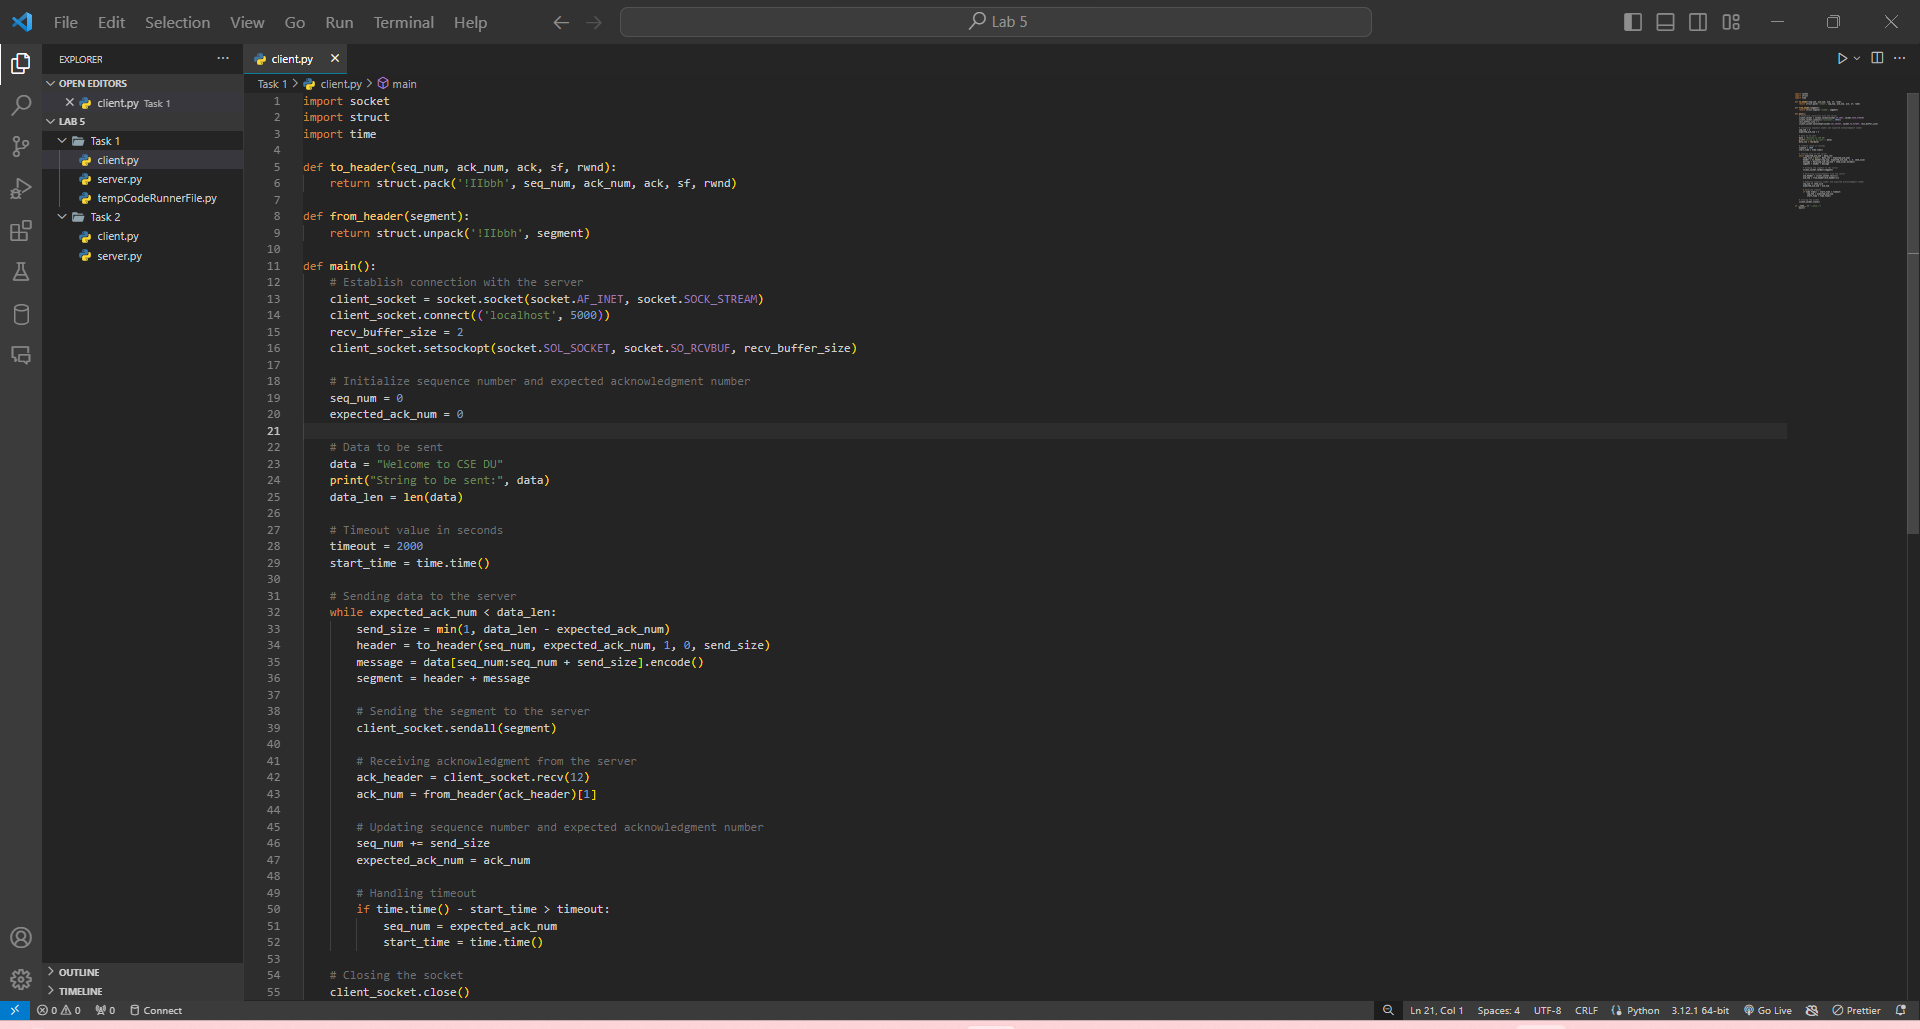
\includegraphics[width=0.8\textwidth]{Task-1-Client.png}
        \caption{Client side code}
        \label{fig:1}
    \end{figure}
    
    \begin{figure}[H]
        \centering
        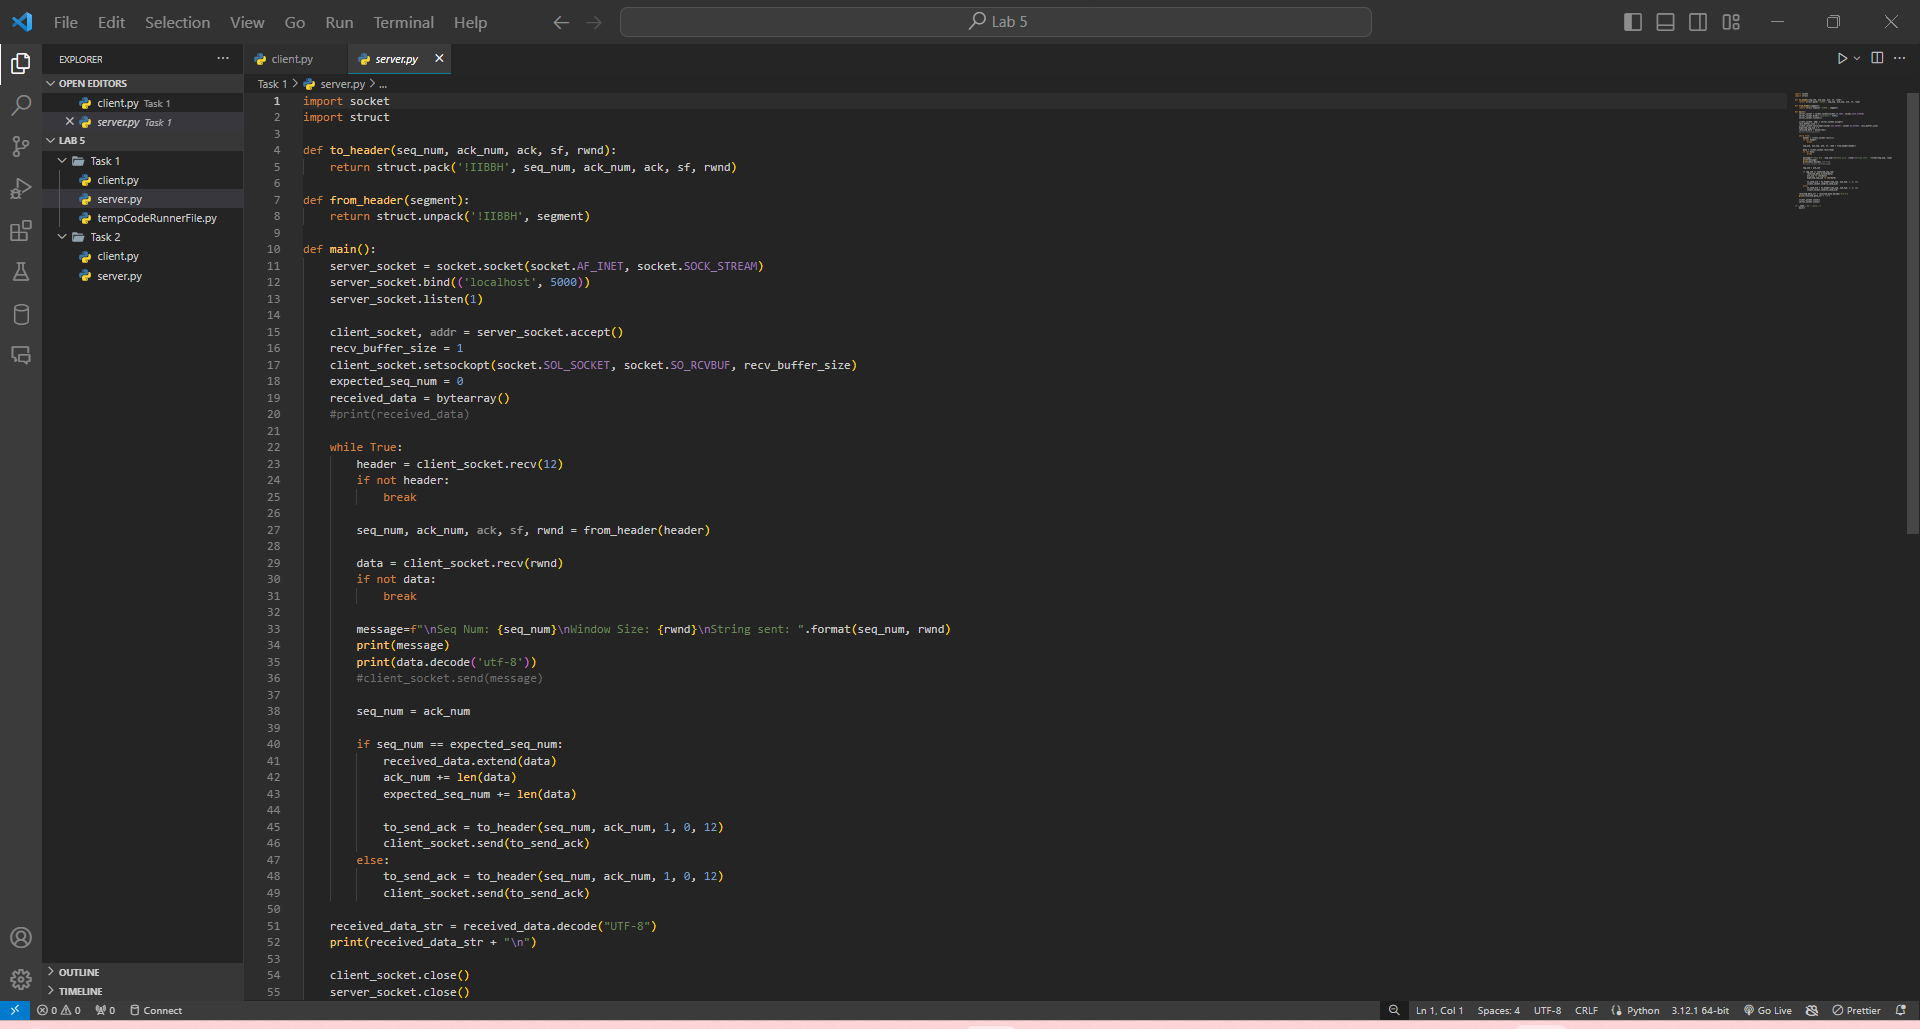
\includegraphics[width=0.8\textwidth]{Task-1-Server.png}
        \caption{Server Side Code}
        \label{fig:2}
    \end{figure}
    \begin{figure}[H]
        \centering
        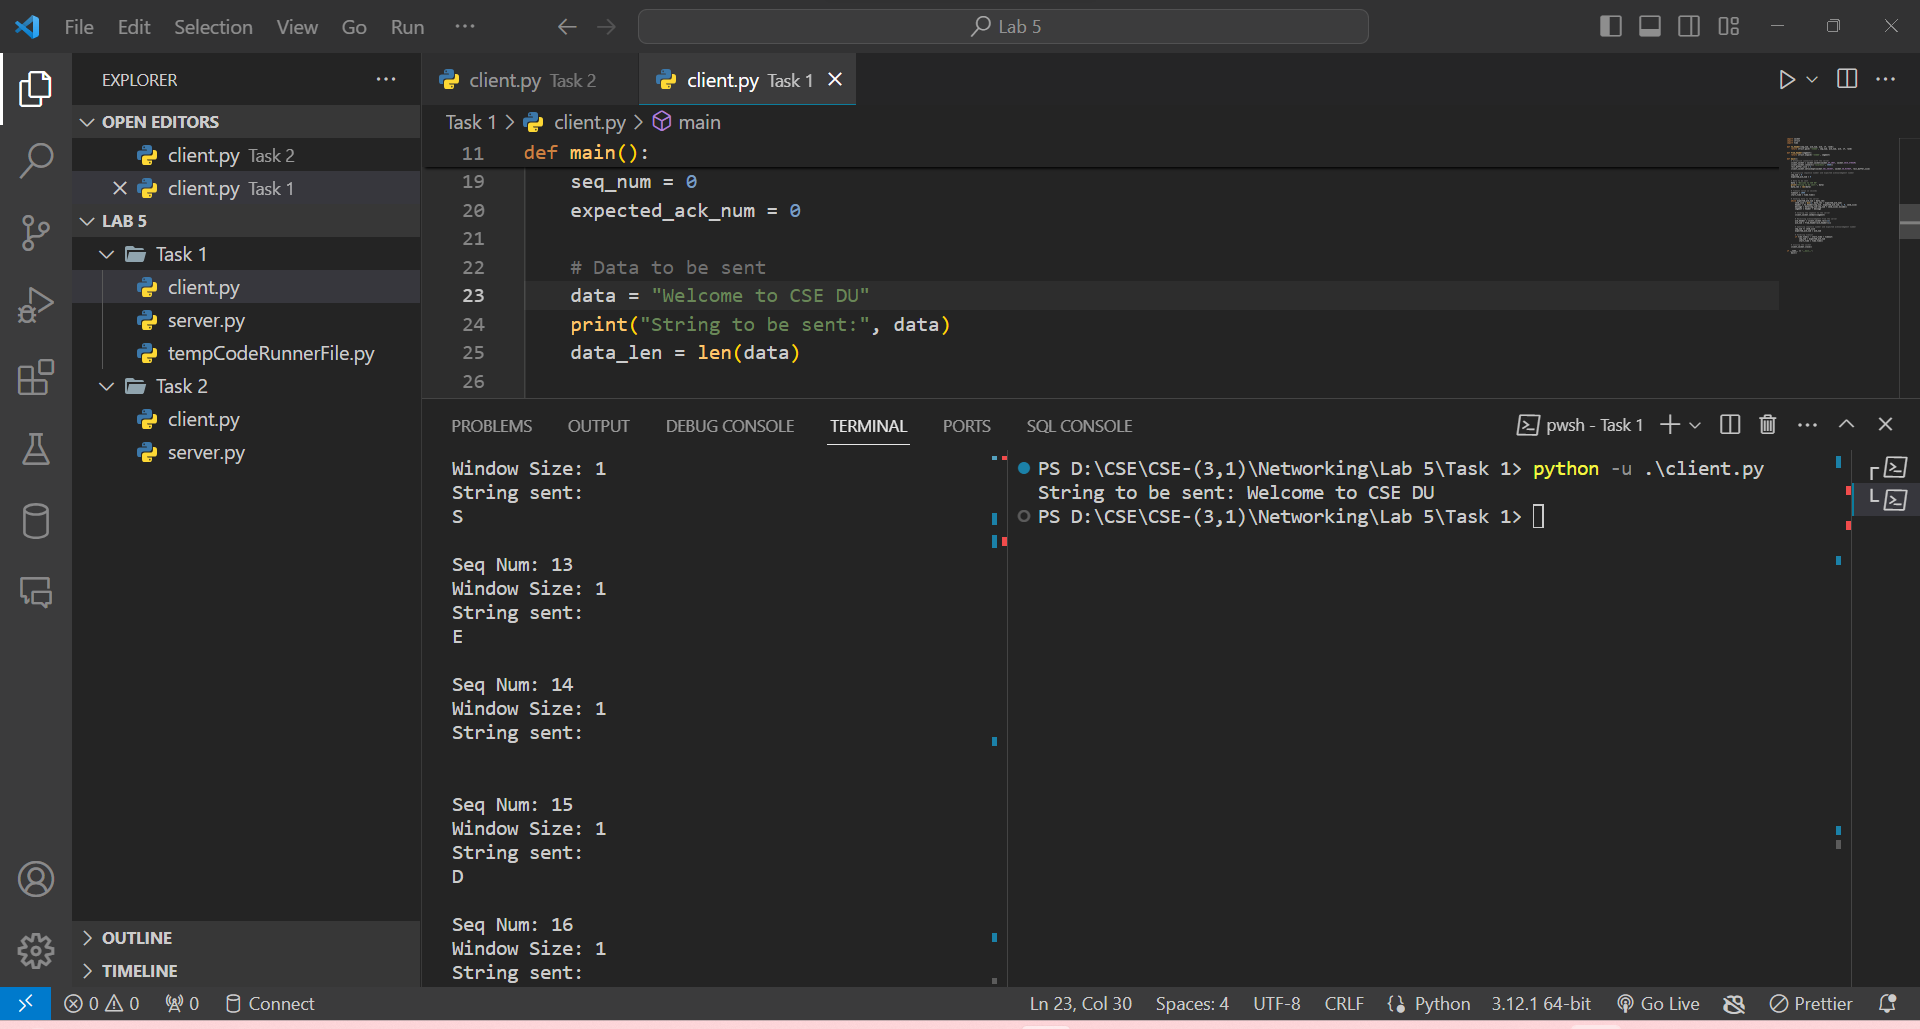
\includegraphics[width=0.8\textwidth]{Lab-5-Task-1.png}
        \caption{Result}
        \label{fig:2}
    \end{figure}
    
    

\end{itemize}

 
\subsection{Task 2}
\begin{itemize}
\item \textbf{Implement reliable data transfer}
 \item Configure the clients to employ the Exponentially Weighted Moving Average (EWMA) equation for determining the TimeOut value. The EWMA equation plays a pivotal role in estimating the Round-Trip Time (RTT) and computing the retransmission timeout (RTO) value.

\item Incorporate the Cumulative Acknowledgment approach into the system, where the receiver acknowledges the highest sequential packet and assumes the receipt of all previous packets up to that designated sequence number.

\item Integrate the fast retransmit algorithm, triggering a retransmission upon detecting three duplicate acknowledgments for the same packet.


\begin{itemize}
    \item \textbf{}
    
  . 
    \begin{figure}[H]
        \centering
        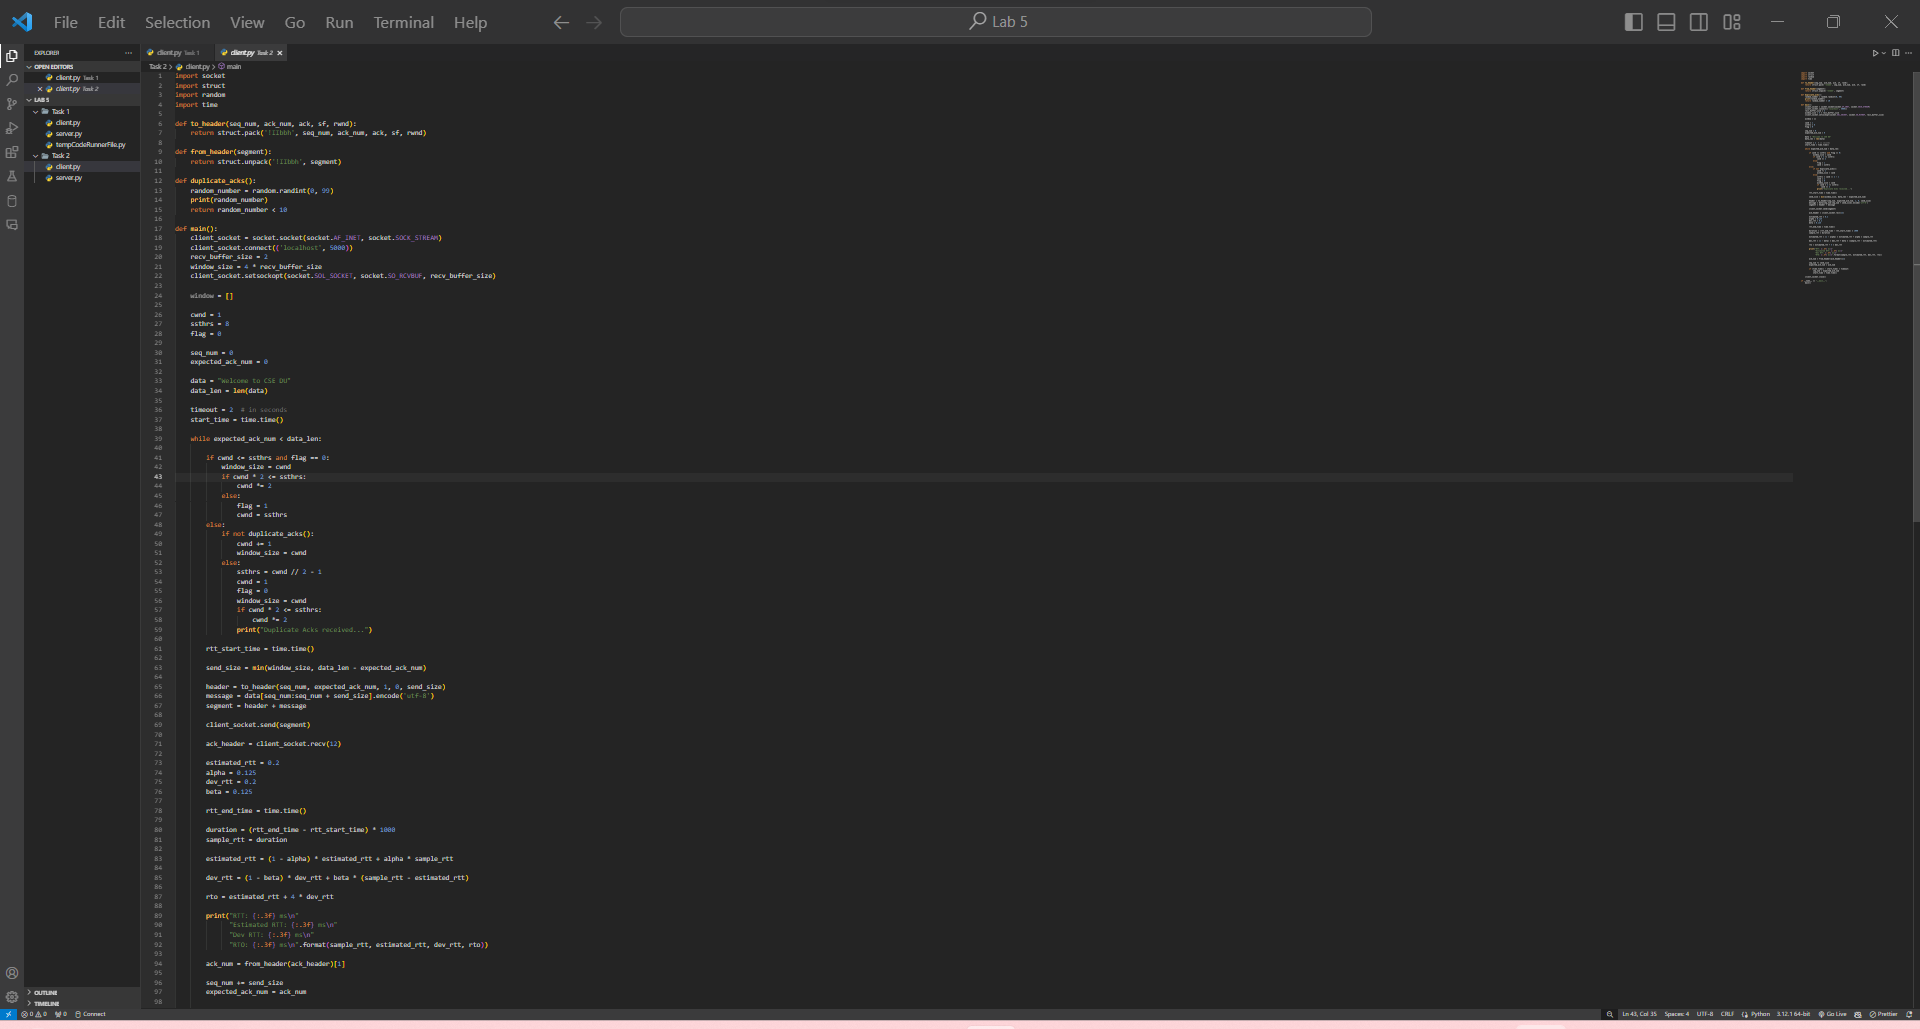
\includegraphics[width=0.8\textwidth]{Task-2-Client.png}
        \caption{Client side code}
        \label{fig:1}
    \end{figure}
    
    \begin{figure}[H]
        \centering
        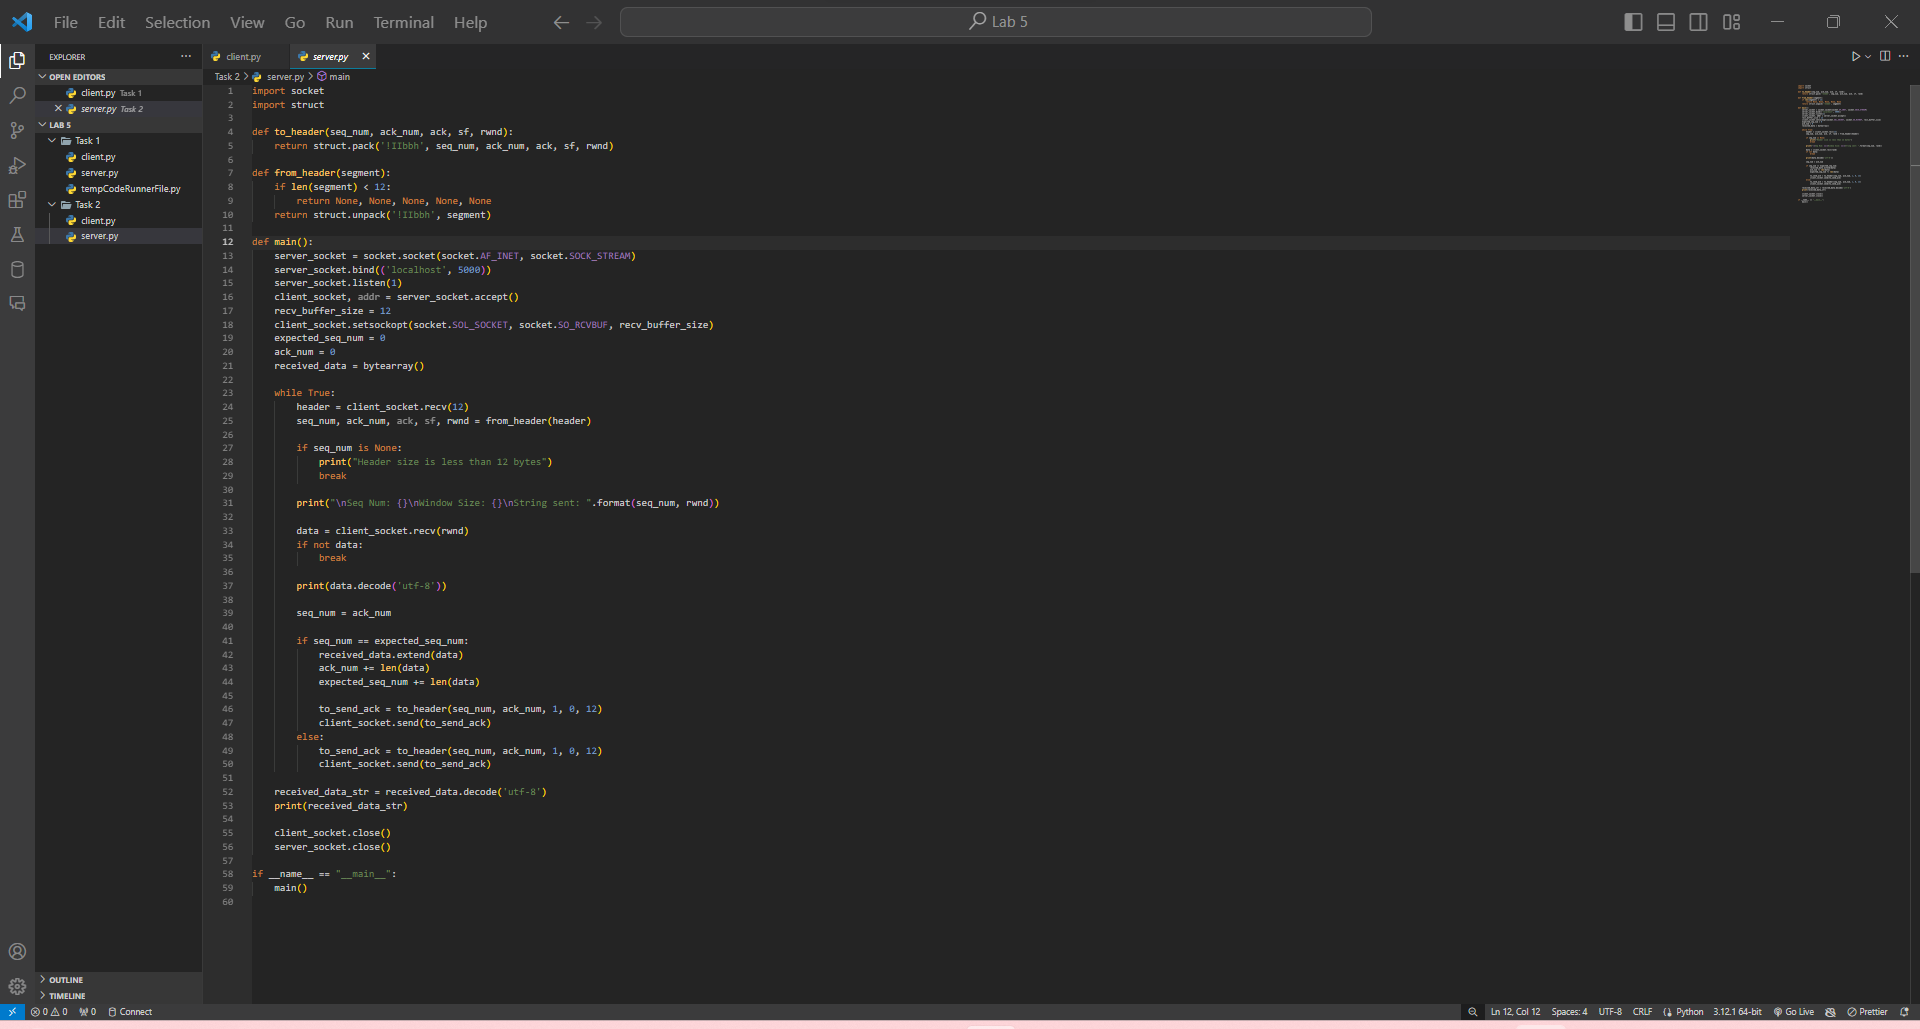
\includegraphics[width=0.8\textwidth]{Task-2-Server.png}
        \caption{Server Side Code}
        \label{fig:2}
    \end{figure}
    

    \begin{figure}[H]
      \centering
      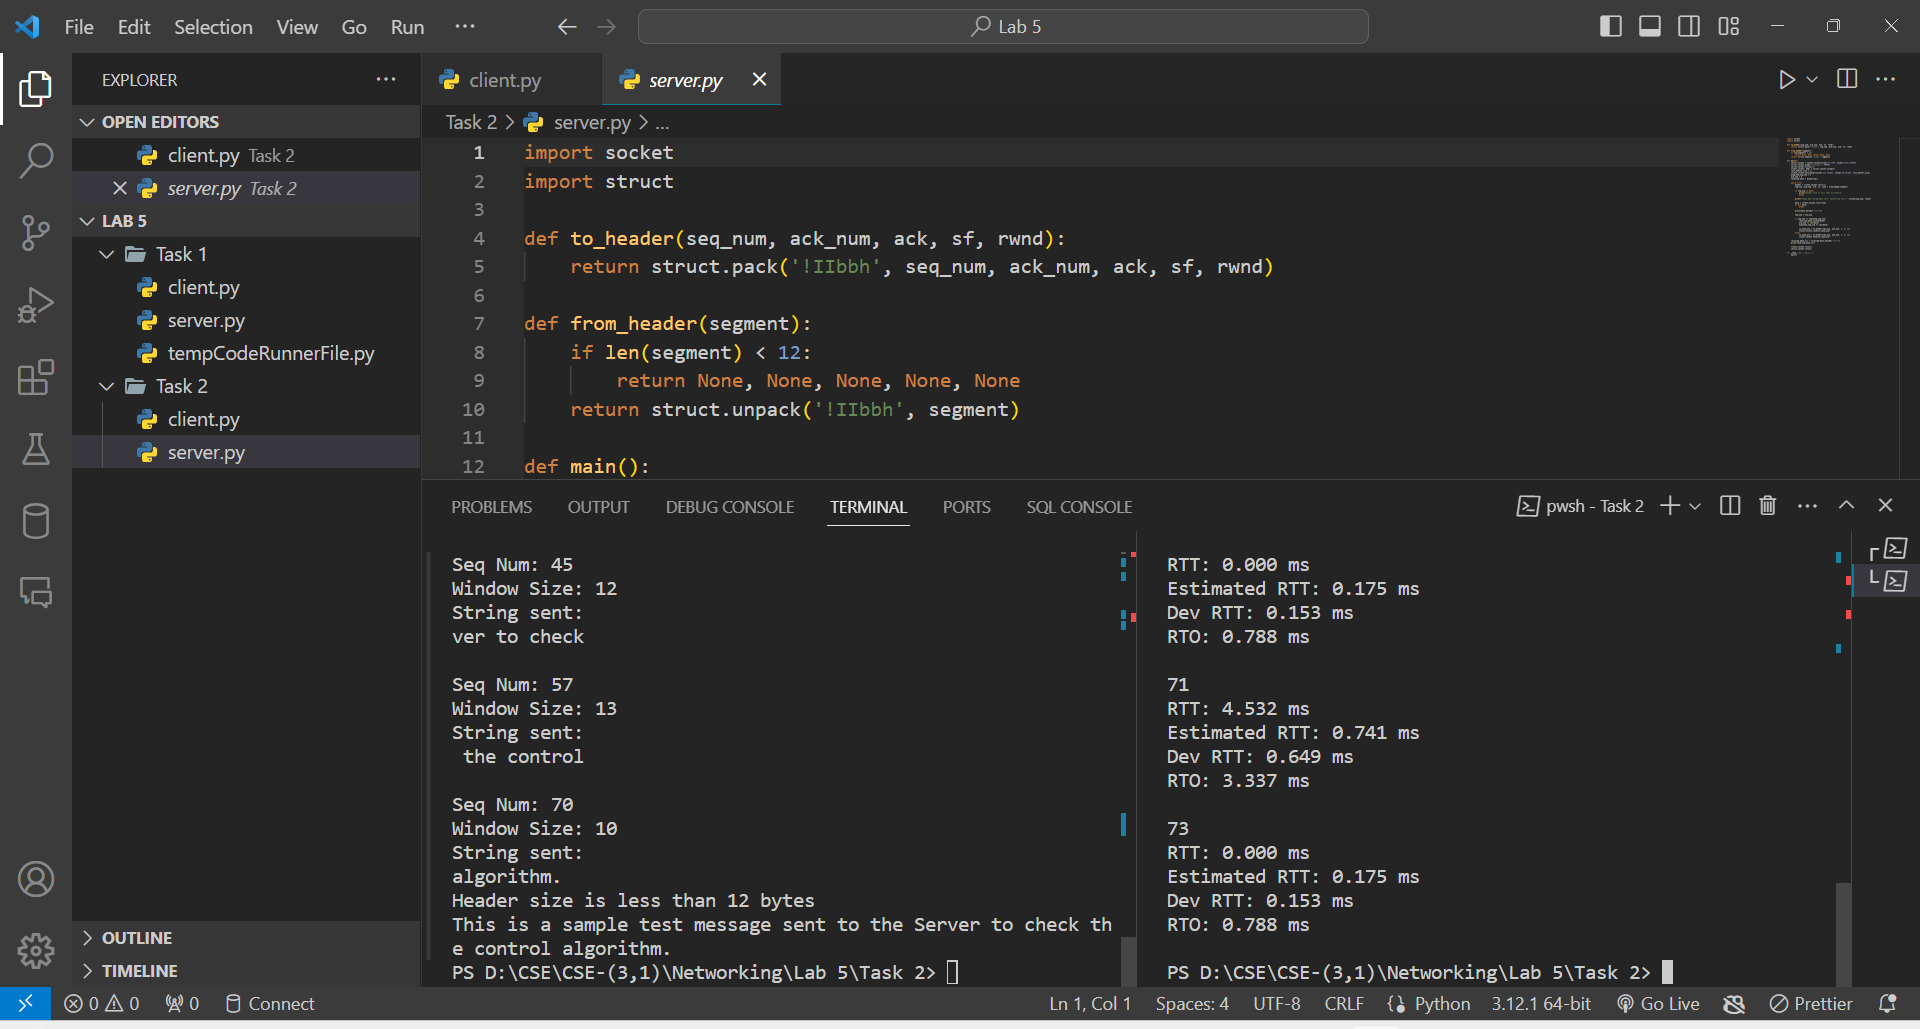
\includegraphics[width=0.8\textwidth]{Lab-5-Task-2.png}
      \caption{Result}
      \label{fig:4}
    \end{figure}

\end{itemize}








\section{Experience}
\begin{enumerate}
    \item  Understanding of the TCP segment structure, particularly the receive window field. This understanding is essential for configuring the server's flow control mechanism accurately 
    \item Timer Management and SampleRTT Calculation
    \item Implementing the Exponentially Weighted Moving Average (EWMA) equation for calculating TimeOut values demands a mathematical understanding and programming proficiency
    \item Considering factors such as clock synchronization and network latency to obtain accurate Round-Trip Time (RTT) measurements for reliable data transfer.
    \item Testing the overall reliability of the data transfer control mechanisms involves comprehensive end-to-end testing.
    
\end{enumerate}





\begin{thebibliography}{1}
  %\bibitem{book} Computer networking: a top-down approach 6th ed.
  \bibitem{Flow Control and Congestion Control} Flow Control and Congestion Control :\url{https://www.geeksforgeeks.org/difference-between-flow-control-and-congestion-control/}
  \bibitem{Difference} Diff erence Between flow and congestion :\url{https://www.javatpoint.com/flow-control-vs-congestion-control}
  \bibitem{Flow Congestion} Feedback-based flow control: \url{https://techdifferences.com/difference-between-flow-control-and-congestion-control.html}
  \bibitem{youtube} Youtube: \url{https://www.youtube.com/watch?v=wQ4_N73duO0&list=PLT5HQnX0CnpUfvgrqBSLkSinFQwrs_6j7}
 
  

 
\end{thebibliography}



\end{document}

